\section{Consultas de subárboles}

\subsection{Preorden}

\begin{frame}
  \frametitle{Consultas de subárboles}

  Supongamos un árbol donde cada nodo tiene un valor numérico. Queremos soportar dos operaciones:

  \begin{itemize}
    \item \texttt{suma(u)}: devuelve la suma de todos los valores del subárbol enraizado en \(u\).
    \item \texttt{cambiar(u, x)}: reemplaza el valor del nodo \(u\) por \(x\).
  \end{itemize}
\end{frame}


\begin{frame}
  \centering
  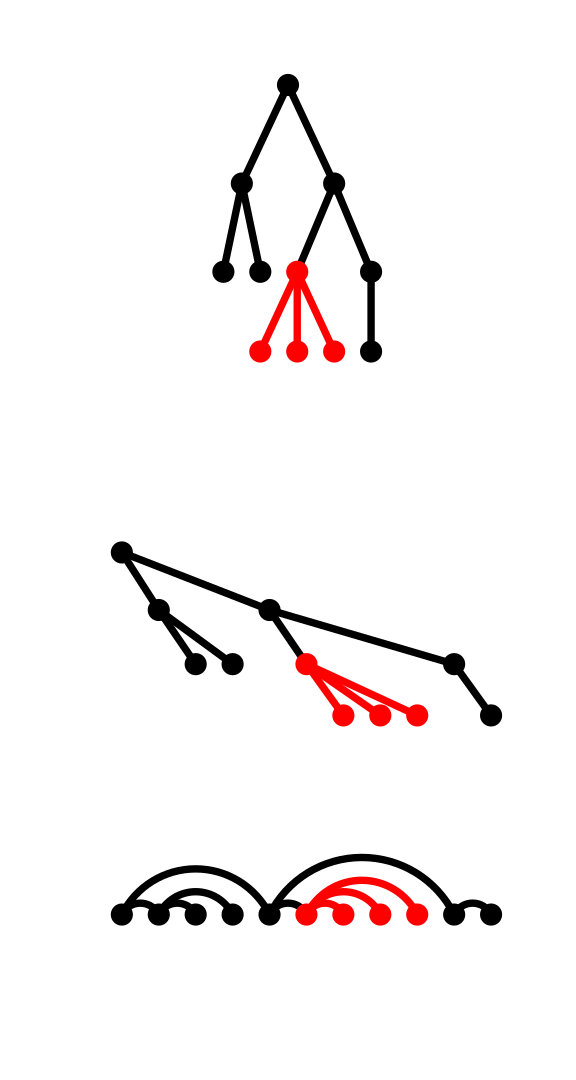
\includegraphics[height=1.05\textheight,keepaspectratio]{fotos/layouts.png}
\end{frame}


\begin{frame}
  \frametitle{Consultas de subárboles: idea}

  Podemos construir el \textbf{preorden} del árbol.

  \vspace{0.75em}

  \begin{itemize}
    \item Propiedad clave: a cada subárbol le corresponde un \textbf{subarray} en el preorden.
    \item Reducimos el problema a consultas en subarrays.
  \end{itemize}
\end{frame}


\begin{frame}[fragile]
  \frametitle{Consultas de subárboles: código}

\begin{lstlisting}
            int lp[maxn], rp[maxn];
            vector<int> pre;
            void dfs(int u, int p) {
                lp[u] = sz(pre);
                pre.push_back(val[u]);
                for (int v : g[u]) if (v != p) {
                    dfs(v, u);
                }
                rp[u] = sz(pre);
            }
            
            int suma(int u) {
                return suma_subarray(lp[u], rp[u]);
            }
\end{lstlisting}
\end{frame}

\begin{frame}
  \frametitle{Consultas de subárboles: observaciones}

  \begin{itemize}
    \item La misma solución sirve para máximos, mínimos, xor, gcd, etc.
    \item Sin embargo, \textbf{no funciona} para cualquier consulta que se nos ocurra.
    \item Por ejemplo: cantidad de números distintos, \texttt{mex} de los números, etc.
  \end{itemize}
\end{frame}
